\documentclass[border=0pt]{standalone}
\usepackage{tikz}
\usetikzlibrary{positioning,shapes,arrows.meta,patterns,calc}
\definecolor{garnet}{HTML}{73000A}
\definecolor{coral}{HTML}{CC2E40}
\definecolor{slate}{HTML}{466A9F}
\definecolor{teal}{HTML}{1F414D}
\definecolor{olive}{HTML}{65780B}
\definecolor{lime}{HTML}{CED318}
\definecolor{gold}{HTML}{A49137}
\begin{document}
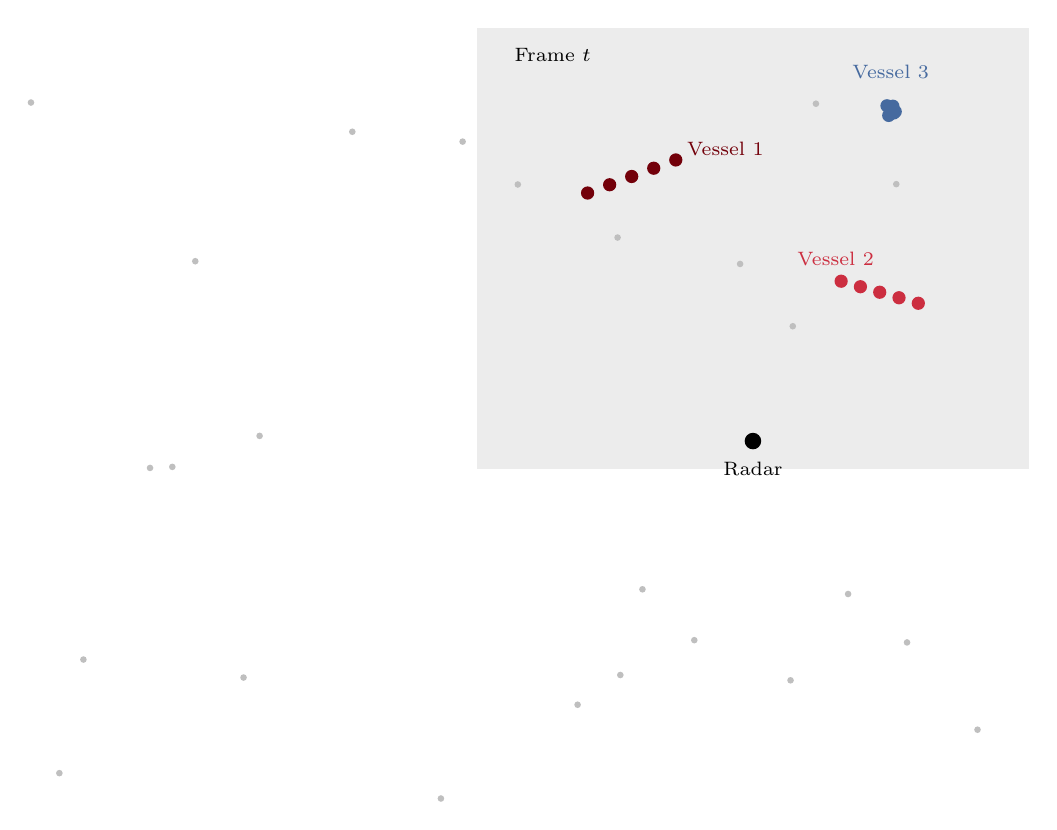
\begin{tikzpicture}[scale=0.7]
    % Background (sea)
    \fill[gray!15] (0,0) rectangle (10,8);
    
    % Radar origin
    \fill[black] (5,0.5) circle (0.15);
    \node[below, font=\scriptsize] at (5,0.3) {Radar};
    
    % Vessel 1 (moving right) - garnet
    \foreach \i in {0,1,2,3,4} {
        \pgfmathsetmacro{\x}{2 + \i*0.4}
        \pgfmathsetmacro{\y}{5 + \i*0.15}
        \fill[garnet] (\x,\y) circle (0.12);
    }
    \node[garnet, font=\scriptsize] at (4.5,5.8) {Vessel 1};
    
    % Vessel 2 (moving left) - coral
    \foreach \i in {0,1,2,3,4} {
        \pgfmathsetmacro{\x}{8 - \i*0.35}
        \pgfmathsetmacro{\y}{3 + \i*0.1}
        \fill[coral] (\x,\y) circle (0.12);
    }
    \node[coral, font=\scriptsize] at (6.5,3.8) {Vessel 2};
    
    % Vessel 3 (stationary) - slate
    \foreach \i in {0,1,2,3,4} {
        \pgfmathsetmacro{\x}{7.5 + rand*0.1}
        \pgfmathsetmacro{\y}{6.5 + rand*0.1}
        \fill[slate] (\x,\y) circle (0.12);
    }
    \node[slate, font=\scriptsize] at (7.5,7.2) {Vessel 3};
    
    % Sea clutter (random noise)
    \foreach \i in {1,...,25} {
        \pgfmathsetmacro{\x}{0.5 + rand*9}
        \pgfmathsetmacro{\y}{0.8 + rand*7}
        \fill[gray!50] (\x,\y) circle (0.06);
    }
    
    % Legend
    \node[right, font=\scriptsize] at (0.5,7.5) {Frame $t$};
\end{tikzpicture}
\end{document}
